% LaTeX-Vorlage Medizintechnik Projektarbeit
% Wintersemster 2009/10
% Alexander Ruppel
% veraendert von Eva Eibenberger 

% %%%%%%%%%%%%%%%%%%%%%%%%%%%%%%%%%%%%%%%%%%%%%%%%%%%%%%
% In dieser Datei muss eigentlich nichts geaendert werden.
% Ausser, einzubettende Dateinamen werden modifiziert.
% %%%%%%%%%%%%%%%%%%%%%%%%%%%%%%%%%%%%%%%%%%%%%%%%%%%%%%

% Gruppe: Nummer der Projektarbeit

% Thema der Projektarbeit
\newcommand{\titel}{Titel der Arbeit}

% Studentenname und Matrikelnummer 
\newcommand{\erster}{Peter Pan}		% Student 1: Vorname Nachname
\newcommand{\mnreins}{1234567}		% Student 1: Matrikelnummer

% in header Spache einstellen!
% LaTeX-Vorlage Medizintechnik Projektarbeit
% Wintersemster 2009/10
% Alexander Ruppel
% veraendert von Eva Eibenberger 

%% Seitenraender
\usepackage[head=12.5mm,headsep=12mm,left=25mm,right=25mm,top=28mm,bottom=20mm]{geometry} 

%% Absatzeinstellungen
\setlength{\parindent}{0em} % Einrueckung neuer Absaetze

%% Kopf- und Fusszeilen
\usepackage{scrlayer-scrpage}
\pagestyle{scrheadings}
\clearscrheadings{} %
\clearscrplain{}	  %
\clearscrheadfoot{} % Kopf- und Fuzeilen werden geloescht
\renewcommand{\headfont}{\normalfont\small}
\ihead{\titel{}}
\ohead{\pagemark}

%% Zeichenkodierung
\usepackage[utf8]{inputenc}
\usepackage{babel,fixltx2e}
\usepackage[T1]{fontenc}

\usepackage[babel]{csquotes}
%% Literaturverzeichnis
%\usepackage[square,authoryear]{natbib}
%\renewcommand{\cite}{\citep}

%% Schriftart
\usepackage{helvet}
\renewcommand{\familydefault}{\sfdefault} % Standardschrift auf sf setzen
\usepackage{textcomp}

%% Tabellen
\usepackage{tabularx}
\usepackage{multirow,multicol}

%% Captions
\usepackage[margin=2em,format=plain,indention=.8em,labelsep=quad,font=small,labelfont=bf,textfont=it]{caption}
\usepackage{breakcites}

%% Mathe & Co
\usepackage{amsmath,amssymb,amsfonts}

%% Grafiken
\usepackage{graphicx}
\graphicspath{{Grafiken/}}
\usepackage{wrapfig}

%% PDF-Optionen
\usepackage[
    bookmarks,
    bookmarksopen=true,
    colorlinks=true,
% diese Farbdefinitionen zeichnen Links im PDF farblich aus
    %linkcolor=red, % einfache interne Verknpfungen
    %anchorcolor=black,% Ankertext
    %citecolor=blue, % Verweise auf Literaturverzeichniseintrge im Text
    %filecolor=magenta, % Verknpfungen, die lokale Dateien ffnen
    %menucolor=red, % Acrobat-Menpunkte
    %urlcolor=cyan, 
% diese Farbdefinitionen sollten fr den Druck verwendet werden (alles schwarz)
    linkcolor=black, % einfache interne Verknpfungen
    anchorcolor=black, % Ankertext
    citecolor=black, % Verweise auf Literaturverzeichniseintrge im Text
    filecolor=black, % Verknpfungen, die lokale Dateien ffnen
    menucolor=black, % Acrobat-Menpunkte
    urlcolor=black, 
    backref, % zurückverweise im Inhaltsverzeichnis auf die Seite
    plainpages=false, % zur korrekten Erstellung der Bookmarks
    pdfpagelabels, % zur korrekten Erstellung der Bookmarks
    hypertexnames=false, % zur korrekten Erstellung der Bookmarks
    linktocpage % Seitenzahlen anstatt Text im Inhaltsverzeichnis verlinken
]{hyperref}

%% Diverses
\usepackage{nameref}
\usepackage{blindtext}
\usepackage{ifthen}

\setlength{\parskip}{\baselineskip}%
\setlength{\parindent}{0pt}%


\begin{document}

% LaTeX-Vorlage Medizintechnik Projektarbeit
% Wintersemster 2009/10
% Alexander Ruppel
% veraendert von Eva Eibenberger 
% veraendert von Paul Stöwer
% veraendert von Mischa Dombrowski

% %%%%%%%%%%%%%%%%%%%%%%%%%%%%%%%%%%%%%%%%%%%%%%%%%%%%%%
% Diese Datei muss NICHT veraendert werden
% %%%%%%%%%%%%%%%%%%%%%%%%%%%%%%%%%%%%%%%%%%%%%%%%%%%%%%

\begin{titlepage}

\begin{center}
Friedrich-Alexander-Universit\"at Erlangen-N\"urnberg\\
Artificial Intelligence in Biomedical Engineering\\
W3-Professur für Image Data Exploration and Analysis\\
Prof.\ B.\ Kainz\\
W3-Professur für Computational Imaging\\
Prof.\ F.\ Knoll\\


\vspace*{9em}

{\huge \textbf{\textsf{Medizintechnik II}}}\\[.3em]
{Projektarbeit}\\[.3em]
{Sommersemester 2022}\\

\vspace*{9em}

{\huge \textbf{\textsf{\titel}}}\\[.7em]
{04.07.2022} %Abgabedatum
\end{center}

\vfill% {
\begin{tabbing}
	\hspace*{5cm} \= Vorname Nachname \hspace*{4em} \= Matrikelnummer \kill
	Studierender:\> \erster \> \mnreins \\
%	\ifthenelse{\equal{\student}{\erster}}{\textbf{\erster} \> \textbf{\mnreins}}{\erster \> \mnreins} \\
%	\ifthenelse{\equal{\student}{\zweiter}}{\textbf{\zweiter} \> \textbf{\mnrzwei}}{\zweiter \> \mnrzwei} \\
%	\ifthenelse{\equal{\student}{\dritter}}{\textbf{\dritter} \> \textbf{\mnrdrei}}{\dritter \> \mnrdrei} \\
%	\ifthenelse{\equal{\student}{\vierter}}{\textbf{\vierter} \> \textbf{\mnrvier}}{\vierter \> \mnrvier} \\
%	\ifthenelse{\equal{\student}{\fuenfter}}{\textbf{\fuenfter} \> \textbf{\mnrfuenf}}{\fuenfter \> \mnrfuenf} \\
\end{tabbing}
%}

\end{titlepage}


% Inhaltsverzeichnis
\tableofcontents
\newpage

% Dateien, die den Text enthalten
\section{Einleitung}%
\label{sec:einleitung}

Dies hier ist ein Blindtext zum Testen von Textausgaben.
Wer diesen Text liest, ist selbst schuld.
Der Text gibt lediglich den Grauwert der Schrift an.
Ist das wirklich so?
Ist es gleichgültig ob ich schreibe:
"Dies ist ein Blindtext" oder "Huardest gefburn"? Kjift mitnichten!
Ein Blindtext bietet mir wichtige Informationen. 
An ihm messe ich die Lesbarkeit einer Schrift, ihre Anmutung,
wie harmonisch die Figuren zueinander stehen und prüfe, wie breit oder schmal sie läuft. 
Ein Blindtext sollte möglichst viele verschiedene Buchstaben enthalten
und in der Originalsprache gesetzt sein. Er muss keinen Sinn ergeben, sollte
aber lesbar sein. Fremdsprachige Texte wie "Lorem ipsum" dienen nicht dem
eigentlichen Zweck, da sie eine falsche Anmutung vermitteln.


Abbildung~\ref{fig:mri} zeigt ein Beispiel für MR-Bilder.
Es gibt viel Literatur zur Normalisierung von Intensitäten in MR-Bildern (z.\,B.~\cite{Jaeger09}). 


\begin{figure}[h]
\centering
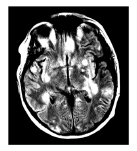
\includegraphics[height=4cm]{Grafiken/jaeger1.png}
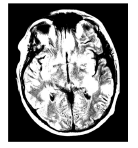
\includegraphics[height=4cm]{Grafiken/jaeger2.png}
\caption{Ein Beispiel für MR-Bilder (entnommen aus \cite{Jaeger09}).}%
\label{fig:mri}
\end{figure}


\section{Segmentierung von Zellen}%
\label{sec:main}

\subsection{Unterthema 1}
\subsection{Unterthema 2}


\section{Fazit}%
\label{sec:fazit} 

Dies hier ist ein Blindtext zum Testen von Textausgaben. Wer diesen Text liest, ist selbst
schuld. Der Text gibt lediglich den Grauwert der Schrift an. Ist das wirklich so? Ist es
gleichg"ultig ob ich schreibe: ``Dies ist ein Blindtext'' oder ``Huardest gefburn''? Kjift 
mitnichten! Ein Blindtext bietet mir wichtige Informationen. An ihm messe ich die Lesbarkeit 
einer Schrift, ihre Anmutung, wie harmonisch die Figuren zueinander stehen
und pr"ufe, wie breit oder schmal sie l"auft. Ein Blindtext sollte m"oglichst viele 
verschiedene Buchstaben enthalten und in der Originalsprache gesetzt sein. Er muss keinen
Sinn ergeben, sollte aber lesbar sein. Fremdsprachige Texte wie ``Lorem ipsum'' dienen nicht 
dem eigentlichen Zweck, da sie eine falsche Anmutung vermitteln.


% Literaturverzeichnis
\newpage
\bibliographystyle{apalike}
\bibliography{Bib/literatur}

\end{document}
